% ═══════════════════════════════════════════════════════════════════════
%  Section 3 — System Architecture
% ═══════════════════════════════════════════════════════════════════════

\section{System Architecture and Technology Stack}
\label{sec:architecture}

\subsection{Technology Stack}

\begin{table}[H]
\centering
\begin{tabular}{p{3.5cm} p{4cm} p{5.5cm}}
    \toprule
    \textbf{Layer} & \textbf{Technology} & \textbf{Rationale} \\
    \midrule
    Operating System & Ubuntu (VM) & Course-provided environment \\
    Database & PostgreSQL 16 & ACID compliance, UUID support, JSONB for audit details \\
    Backend Framework & Python / FastAPI & Async support, automatic OpenAPI docs, dependency injection \\
    Frontend Framework & React 18 + Vite & Component-based UI, fast HMR, modern build tooling \\
    Web Server & Nginx & Reverse proxy, TLS termination, static asset serving \\
    Containerization & Docker + Docker Compose & Reproducible builds, CI/CD pipeline \\
    CI/CD & GitHub Actions & Automated lint, test, build, and deploy \\
    \bottomrule
\end{tabular}
\caption{Technology stack overview.}
\end{table}

\subsection{Architecture Diagram}

The system follows a standard three-tier architecture:

\begin{center}
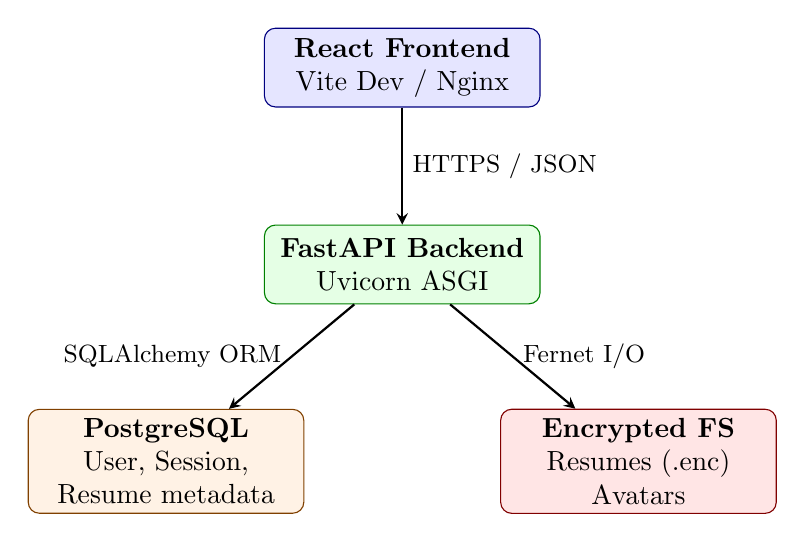
\begin{tikzpicture}[
    box/.style={draw, rounded corners, minimum width=3.5cm, minimum height=1cm, align=center, fill=#1!10, draw=#1!50!black},
    arrow/.style={->, thick, >=stealth}
]
    % Client
    \node[box=blue] (client) at (0, 6) {\textbf{React Frontend}\\Vite Dev / Nginx};

    % API
    \node[box=green] (api) at (0, 3.5) {\textbf{FastAPI Backend}\\Uvicorn ASGI};

    % Database
    \node[box=orange] (db) at (-3, 1) {\textbf{PostgreSQL}\\User, Session,\\Resume metadata};

    % Filesystem
    \node[box=red] (fs) at (3, 1) {\textbf{Encrypted FS}\\Resumes (.enc)\\Avatars};

    % Arrows
    \draw[arrow] (client) -- node[right, font=\small] {HTTPS / JSON} (api);
    \draw[arrow] (api) -- node[left, font=\small] {SQLAlchemy ORM} (db);
    \draw[arrow] (api) -- node[right, font=\small] {Fernet I/O} (fs);
\end{tikzpicture}
\end{center}

\subsection{Backend Architecture}

The FastAPI backend is organized into clearly separated modules:

\begin{itemize}
    \item \texttt{app/routers/} — API endpoint handlers (auth, users, resumes, admin, profile)
    \item \texttt{app/models/} — SQLAlchemy ORM models (User, Session, Resume, AuditLog, Education, etc.)
    \item \texttt{app/schemas/} — Pydantic request/response schemas with input sanitization
    \item \texttt{app/security/} — Cryptographic primitives (password hashing, JWT, TOTP, file encryption, CSRF)
    \item \texttt{app/dependencies.py} — Authentication and RBAC dependency injection
    \item \texttt{app/config.py} — Environment-based configuration
\end{itemize}

\subsection{Frontend Architecture}

The React frontend is built with Vite and follows a component-based architecture:

\begin{itemize}
    \item \texttt{src/pages/} — Page-level components (Landing, Login, Register, Dashboard, Profile, Resumes, AdminPanel)
    \item \texttt{src/components/} — Reusable UI components (Navbar, Icons, Toast, ConfirmDialog)
    \item \texttt{src/context/} — React Context providers (AuthContext, ThemeContext, ToastProvider, ConfirmProvider)
    \item \texttt{src/data/} — Static data (curated skills list)
\end{itemize}

\subsection{Database Schema}

Key tables in the PostgreSQL database:

\begin{table}[H]
\centering
\begin{tabular}{p{3.5cm} p{9.5cm}}
    \toprule
    \textbf{Table} & \textbf{Purpose} \\
    \midrule
    \texttt{users} & User accounts with Argon2id-hashed passwords, TOTP secrets (Fernet-encrypted), role, suspension status \\
    \texttt{sessions} & JWT session tracking with refresh token JTI, device fingerprint, revocation status \\
    \texttt{resumes} & Resume metadata (original filename, stored path, encryption key version) \\
    \texttt{audit\_logs} & Immutable security event log with action, IP, timestamp, JSONB details \\
    \texttt{used\_otps} & TOTP replay prevention — tracks used codes per time window \\
    \texttt{user\_education} & Education entries (institution, degree, field, years) \\
    \texttt{user\_experience} & Work experience entries (company, title, dates, description) \\
    \texttt{user\_skills} & Skills with unique constraint per user \\
    \bottomrule
\end{tabular}
\caption{Database schema overview.}
\end{table}

\subsection{Deployment Pipeline}

\begin{enumerate}
    \item \textbf{CI (Continuous Integration)} — GitHub Actions runs on every push to \texttt{main}:
    \begin{itemize}
        \item Backend: Python 3.11 setup, \texttt{ruff} linting, \texttt{pytest} unit tests
        \item Frontend: Node 20 setup, ESLint, production build verification
    \end{itemize}
    \item \textbf{CD (Continuous Deployment)} — After CI passes:
    \begin{itemize}
        \item Builds Docker images for backend and frontend
        \item Pushes to GitHub Container Registry (GHCR)
        \item Tagged with commit SHA and \texttt{latest}
    \end{itemize}
\end{enumerate}
